\chapter{Hamiltonian Path/Cycle}
Ajur was walking with Jura thinking how a walk could be named after him. Rishnak found Ajur to be an interesting person to discuss puzzles related to Graph Theory. After the Eulerian Walk, Rishnak thought of another closely related walk- namely Hamiltonian Path and Hamiltonian Cycle. A Hamiltonian Path is a path in which all the vertices are visited exactly once. 
The length of a path is the number of edges in that path. A Hamiltonian path in a graph with $n$ vertices will have a path length of $n-1$, A Hamiltonian cycle is a cycle that visits each vertex once and only once. The length of Hamiltonian Cycle in a graph with $n$ vertices will have a length of $n$. Rishnak asked Ajur whether there is a Hamiltonian Cycle in the following graph Figure \ref{5g1},
\begin{figure}
\begin{center}
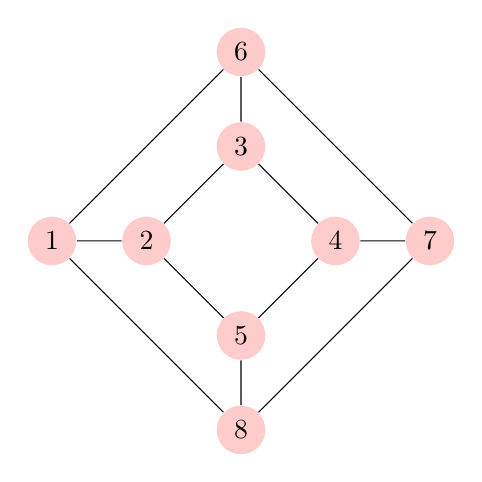
\begin{tikzpicture}
  [scale=.6,auto=left,every node/.style={circle,fill=red!20}]
  \node (n1) at (1,7) {1};
  \node (n2) at (3,7)  {2};
  \node (n4) at (7,7) {4};
  \node (n7) at (9,7)  {7};
  \node (n6) at (5,11)  {6};
   \node (n3) at (5,9) {3};
   \node (n5) at (5,5) {5};
   \node (n8)  at (5,3) {8};
  \foreach \from/\to in {n1/n2,n2/n3,n3/n4,n4/n5,n5/n2,n1/n6,
  n6/n7, n7/n8, n8/n1, n3/n6, n4/n7, n5/n8}
    \draw (\from) -- (\to);

\end{tikzpicture}
\caption{ Cube Graph }\label{5g1}
\end{center}
\end{figure}

Ajur thought about for a few seconds and he drew the Hamiltonian cycle of Figure \ref{5g1} in Figure \ref {5g2}

\begin{figure}
\begin{center}
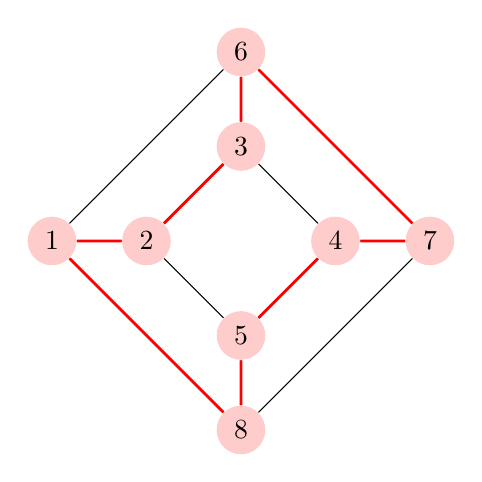
\begin{tikzpicture}
  [scale=.6,auto=left,every node/.style={circle,fill=red!20}]
  \node (n1) at (1,7) {1};
  \node (n2) at (3,7)  {2};
  \node (n4) at (7,7) {4};
  \node (n7) at (9,7)  {7};
  \node (n6) at (5,11)  {6};
   \node (n3) at (5,9) {3};
   \node (n5) at (5,5) {5};
   \node (n8)  at (5,3) {8};
  \foreach \from/\to in {n1/n2,n2/n3,n3/n4,n4/n5,n5/n2,n1/n6,
  n6/n7, n7/n8, n8/n1, n3/n6, n4/n7, n5/n8}
    \draw (\from) -- (\to);
\path[line width=0.35mm,red] (n1) edge (n2)
(n2) edge (n3)
(n3) edge (n6)
(n6) edge (n7)
(n7) edge (n4)
(n4) edge (n5)
(n5) edge (n8)
(n8) edge (n1);
\end{tikzpicture}
\caption{ Cube Graph with Hamiltonian  Cycle marked in thick edges}\label{5g2}
\end{center}
\end{figure}

Rishnak mentioned that the Hamiltonian cycle problem started
when mathematician Hamilton wanted a cycle to visit 
all the vertices of a Dodecahedron (another platonic solid, like cube) which has 20 vertices and 30 edges. 
Rishnak asked Ajur whether there is a Hamiltonian Cycle in this graph Figure \ref{5g3}. Rishnak added that this is a well known graph known as Petersen Graph.

\begin{figure}
\begin{center}
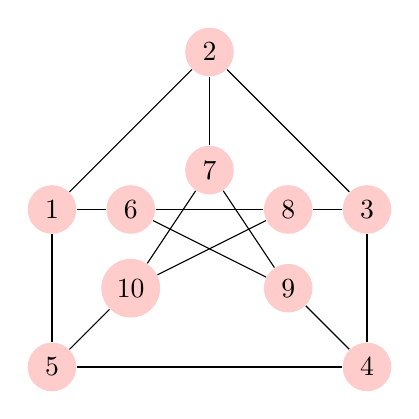
\begin{tikzpicture}
  [scale=.5,auto=left,every node/.style={circle,fill=red!20}]
  \node (n1) at (1,7) {1};
  \node (n2) at (5,11)  {2};
  \node (n3) at (9,7)  {3};
  \node (n4) at (9,3) {4};
  \node (n5) at (1,3) {5};
  \node (n6) at (3,7)  {6};
  \node (n7) at (5,8) {7};
  \node (n8)  at (7,7) {8};
  \node (n9) at (7,5) {9};
  \node (n10) at  (3,5) {10};
 
  \foreach \from/\to in {n1/n2,n2/n3,n3/n4,n4/n5,n5/n1,n1/n6,
  n2/n7, n3/n8, n4/n9, n5/n10, n6/n8, n8/n10, n10/n7,n7/n9,n9/n6}
    \draw (\from) -- (\to);

\end{tikzpicture}
\caption{ Petersen Graph with 10 vertices and 15 edges }\label{5g3}
\end{center}
\end{figure}
Ajur thought for a while and he was not able to construct a Hamiltonian cycle. He however, was able to find a 
Hamiltonian Path. So he drew the following Figure \ref{5g4}


\begin{figure}
\begin{center}
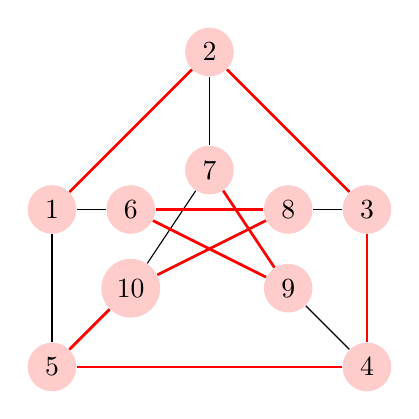
\begin{tikzpicture}
  [scale=.5,auto=left,every node/.style={circle,fill=red!20}]
  \node (n1) at (1,7) {1};
  \node (n2) at (5,11)  {2};
  \node (n3) at (9,7)  {3};
  \node (n4) at (9,3) {4};
  \node (n5) at (1,3) {5};
  \node (n6) at (3,7)  {6};
  \node (n7) at (5,8) {7};
  \node (n8)  at (7,7) {8};
  \node (n9) at (7,5) {9};
  \node (n10) at  (3,5) {10};
 
  \foreach \from/\to in {n1/n2,n2/n3,n3/n4,n4/n5,n5/n1,n1/n6,
  n2/n7, n3/n8, n4/n9, n5/n10, n6/n8, n8/n10, n10/n7,n7/n9,n9/n6}
    \draw (\from) -- (\to);
\path[line width=0.35mm,red]
(n1) edge (n2)
(n2) edge (n3)
(n3) edge (n4)
(n4) edge (n5)
(n5) edge (n10)
(n10) edge (n8)
(n8) edge (n6)
(n6) edge (n9)
(n9) edge (n7);

\end{tikzpicture}
\caption{ Petersen Graph with a Hamiltonian Path}\label{5g4}
\end{center}
\end{figure}
Rishnak assured Ajur that Petersen Graph does not have a Hamiltonian Cycle. For testing whether a graph has an Eulerian Cycle or not can easily be tested (the degree of every vertex has to be even), there is no easy method for testing whether a given graph has a Hamiltonian cycle. 
Rishnak continued that there is a special class of graphs called bipartite graphs where every cycle is of even length. The vertex set can be partitioned into two sets $A$ and $B$, such that every edge in such a graph has one end vertex in $A$ and the other end vertex in $B$. Rishnak showed an example Figure \ref{5g5}. Ajur immediately said that all the cycles oare of even lengths (4 and 6). Rishnak asked Ajur what the two vertex partitions are (all the edges go from one partition to the other). Ajur thought about it for a few seconds and said one partition contains 1, 3, 5 and the other partition contains the vertices 2, 4 and 6. Ajur also mentioned that this graph has a Hamiltonian cycle. Ajur exclaimed that every tree is a bipartite graph too , as tree contains no cycles (or cycles of length 0 - we know that 0 is an even number!). Rishnak reminded Ajur that since tree does not have cycles and hence Hamiltonian cycles. 
Ajur wanted to show that he has understood the concept of bipartite graphs. So he drew a graph - see Figure \ref{5g6} that does not a Hamiltonian cycle. Ajur explained why this graph does not have a Hamiltonian cycle. If there were a Hamiltonian cycle, the vertices in the cycle have to alternate between the two vertex partitions. But one vertex partition has two vertices and the other vertex partition has three vertices. Rishnak smiled and appreciated Ajur's logical thinking.

\begin{figure}
\begin{center}
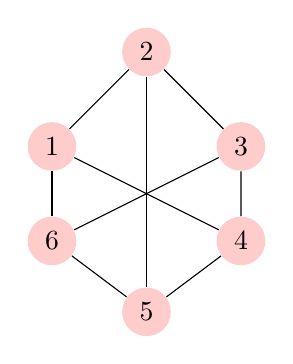
\begin{tikzpicture}
  [scale=.3,auto=left,every node/.style={circle,fill=red!20}]
  \node (n1) at (1,7) {1};
  \node (n2) at (5,11)  {2};
  \node (n3) at (9,7)  {3};
  \node (n4) at (9,3) {4};
  \node (n5) at (5,0)  {5};
  \node (n6) at (1,3) {6};
  
   \foreach \from/\to in {n1/n2,n2/n3,n3/n4,n4/n5,n5/n6,n1/n6,
  n2/n5, n6/n3,n1/n4}
    \draw (\from) -- (\to);
    \end{tikzpicture}
\caption{ A Bipartite Graph with 6 vertices and 9 edges}\label{5g5}
\end{center}
\end{figure}
\begin{figure}
\begin{center}
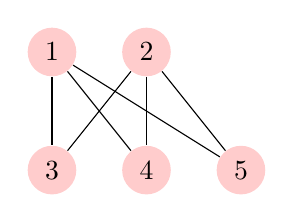
\begin{tikzpicture}
  [scale=.3,auto=left,every node/.style={circle,fill=red!20}]
  \node (n1) at (1,7) {1};
  \node (n2) at (5,7)  {2};
  \node (n3) at (1,2)  {3};
  \node (n4) at (5,2) {4};
  \node (n5) at (9,2)  {5};
 
  
   \foreach \from/\to in {n1/n3,n1/n4,n1/n5,n2/n3,n2/n4,n2/n5}
    \draw (\from) -- (\to);
    \end{tikzpicture}
\caption{ A Bipartite Graph with 5 vertices and 6 edges}\label{5g6}
\end{center}
\end{figure}